In this research the primary fault model of concern is the ``cell-aware fault model.''
To differentiate this from other types of fault models, consider the locations at which faults can occur. 
For instance, consider the example of a stuck-at fault in Section \ref{sec:intr}.
As was stated there, a stuck at fault can only occur on the interconnects between logic gates. 
Perhaps a more technically correct way of saying this is: defects can only be modeled as occurring on logic nets. 
As another example, examine Figure \ref{fig:bf} which represents a couple potential faults using the bridging fault model.

\begin{figure}[h!]
\centering
\caption{Example of a Bridging Fault\label{fig:bf}}
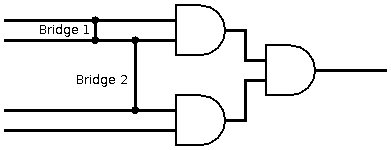
\includegraphics[scale=0.5]{Figures/bf.png}
\end{figure}  

Notice again that the faults in this example occur on electrical nets outside of the logic cells. 
To extend the analogy, these types of fault models could be labeled as ``cell-unaware faults.''
This is because the defects are all modeled without respect to the internals of each of the standard cells in the circuit. 
This is not to say that faults can only occur outside the gates.
Many faults occur within logic cells, but are able to be effectively modeled and detected by fault models which represent faults outside standard cells. 
In other words, even though the manufacturing defect doesn't produce a circuit exactly like the one seen in Figures \ref{fig:safault} and \ref{fig:bf}, these faults can be effectively modeled as and tested for by thinking of the circuit as shown. 

Unfortunately, the disregard for the internals of a standard cell produce a large class of faults which will not be considered. 
Or rather, will not be targeted during ATPG for a fault model that only considers the electrical nets between gates.
To get a better feel for cell-aware type faults we will perform cell-aware type ATPG for the NOR gate in Figure \ref{fig:nor}. 
To discover the internal faults that will not be tested for by a traditional fault model, we will first perform ATPG with regards to the traditional model.
For this example (and in this research) we use the stuck-at fault model.

\begin{figure}[h!]
\centering
\caption{Nor gate for stuck-at ATPG Example\label{fig:nor}}
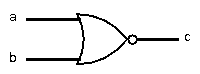
\includegraphics[scale=0.5]{Figures/nor.png}
\end{figure}
\begin{center}
\begin{tabular}{ c c | c }
    a&b&c \\
    \hline
    0&0&1 \\
    0&1&0 \\
    1&0&0 \\
    1&1&0 \\
\end{tabular}
\end{center}

There are six potential stuck-at faults that we need to test for: a stuck-at 0, a stuck-at 1, b stuck-at 0, b stuck-at 1, c stuck-at 0, and c stuck-at 1. 
To derive the stuck at test set, let us find the smallest set of patterns that will test for each of these faults. 
To test for a fault, we must first excite the fault, and then observe the net at the output of the circuit ( This is done with the use of the Boolean derivative). 
To excite a fault, we force a net to the opposite value than what it is stuck at. 


\begin{align*}
    T_{a/0} &= a\frac{\delta a}{\delta c} = a\overline{b} \\
    T_{a/1} &= \overline{a}\frac{\delta a}{\delta c} = \overline{a}\overline{b} \\
    T_{b/0} &= b\frac{\delta b}{\delta c} = b\overline{a} \\ 
    T_{b/1} &= \overline{b}\frac{\delta b}{\delta c} = \overline{b}\overline{a} \\ 
    T_{c/0} &= \overline{a}\overline{b}\frac{\delta c}{\delta c} = \overline{a}\overline{b} \\ 
    T_{c/1} &= (\overline{a}b + a\overline{b} + ab)\frac{\delta c}{\delta c} = (\overline{a}b + a\overline{b} + ab) 
\end{align*}

To minimize the test set, the ATPG tool would then na\"ively suggest:

\begin{equation}
T=\{a\overline{b}, \overline{a}b, \overline{a}\overline{b}\}
\end{equation}

With this test set, we can effectively test for all stuck-at faults in our small example circuit. 
But we are simply \textit{modeling} faults as occurring on lines outside of logic gates.
What if the real fault is inside the circuit, and can only be detected with the test pattern $ab$ (or a = 1 and b =1)? 
Figure \ref{fig:caf} illustrates a cell aware fault inside a nor gate, and describes the test pattern that detects it. 

\begin{figure}[h!]
\centering
\caption{Example of a Cell-Aware Fault\label{fig:caf}}
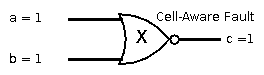
\includegraphics[scale=0.5]{Figures/caf.png}
\end{figure}  

A good understanding of the cell-aware fault model is essential for understanding parts of our methodology.
This example is a good introduction to cell-aware faults.
Ron Press posted an excellent tutorial explaining these faults online in 2012\cite{ronpress}.